\chapter{Data Acquisition and Computing for the Near Detector System} % (NDS) DAQ and Computing}
\label{ch:nd-gdaq}

\section{Introduction}
\label{sec:nd-gdaq-intro}

The Near Detector System (i.e., overall NDS) Data Acquisition system (NDS-DAQ) collects raw data from each NDS detector's
individual DAQ, %in the NDS , 
issues global \fixme{global in what sense here?} triggers, adds precision timing 
data from a global positioning system (GPS), and builds events. %Each NDS detector has its own data acquisition system that connects to the NDS-DAQ.

The NDS-DAQ is made up of two parts: NDS Master DAQ (NDS-MDAQ) and the Beamline Measurements 
DAQ (BLM-DAQ). A third component, the Near Neutrino Detector DAQ (NND-DAQ) is part of the Near Neutrino Detector system (in contrast to the BLM-DAQ) and is 
connected to the NDS Master DAQ. It is described in Section~\ref{sec:nd:nnd:daq}.
Figure~\ref{fig:DAQ_Block} shows a block diagram for the NDS-DAQ.

\fixme{The composition of the nds-daq must be a management thing only?  In the diagram the nnd-daq and the blm-daq appear to have identical connections to the master daq. We should clarify.}

\begin{cdrfigure}[Near Detector System DAQ block diagram]{DAQ_Block}{Near Detector System DAQ block diagram: The NDS-DAQ consists 
of two parts: NDS Master DAQ (green blocks) and Beamline Measurement DAQ (yellow summary 
block). The NearSite Detectors DAQ (orange block) is described in a separate chapter. The 
NDS-DAQ connects to other sections of the LBNE project, shown here in other colors (blue, 
light red, tan).}
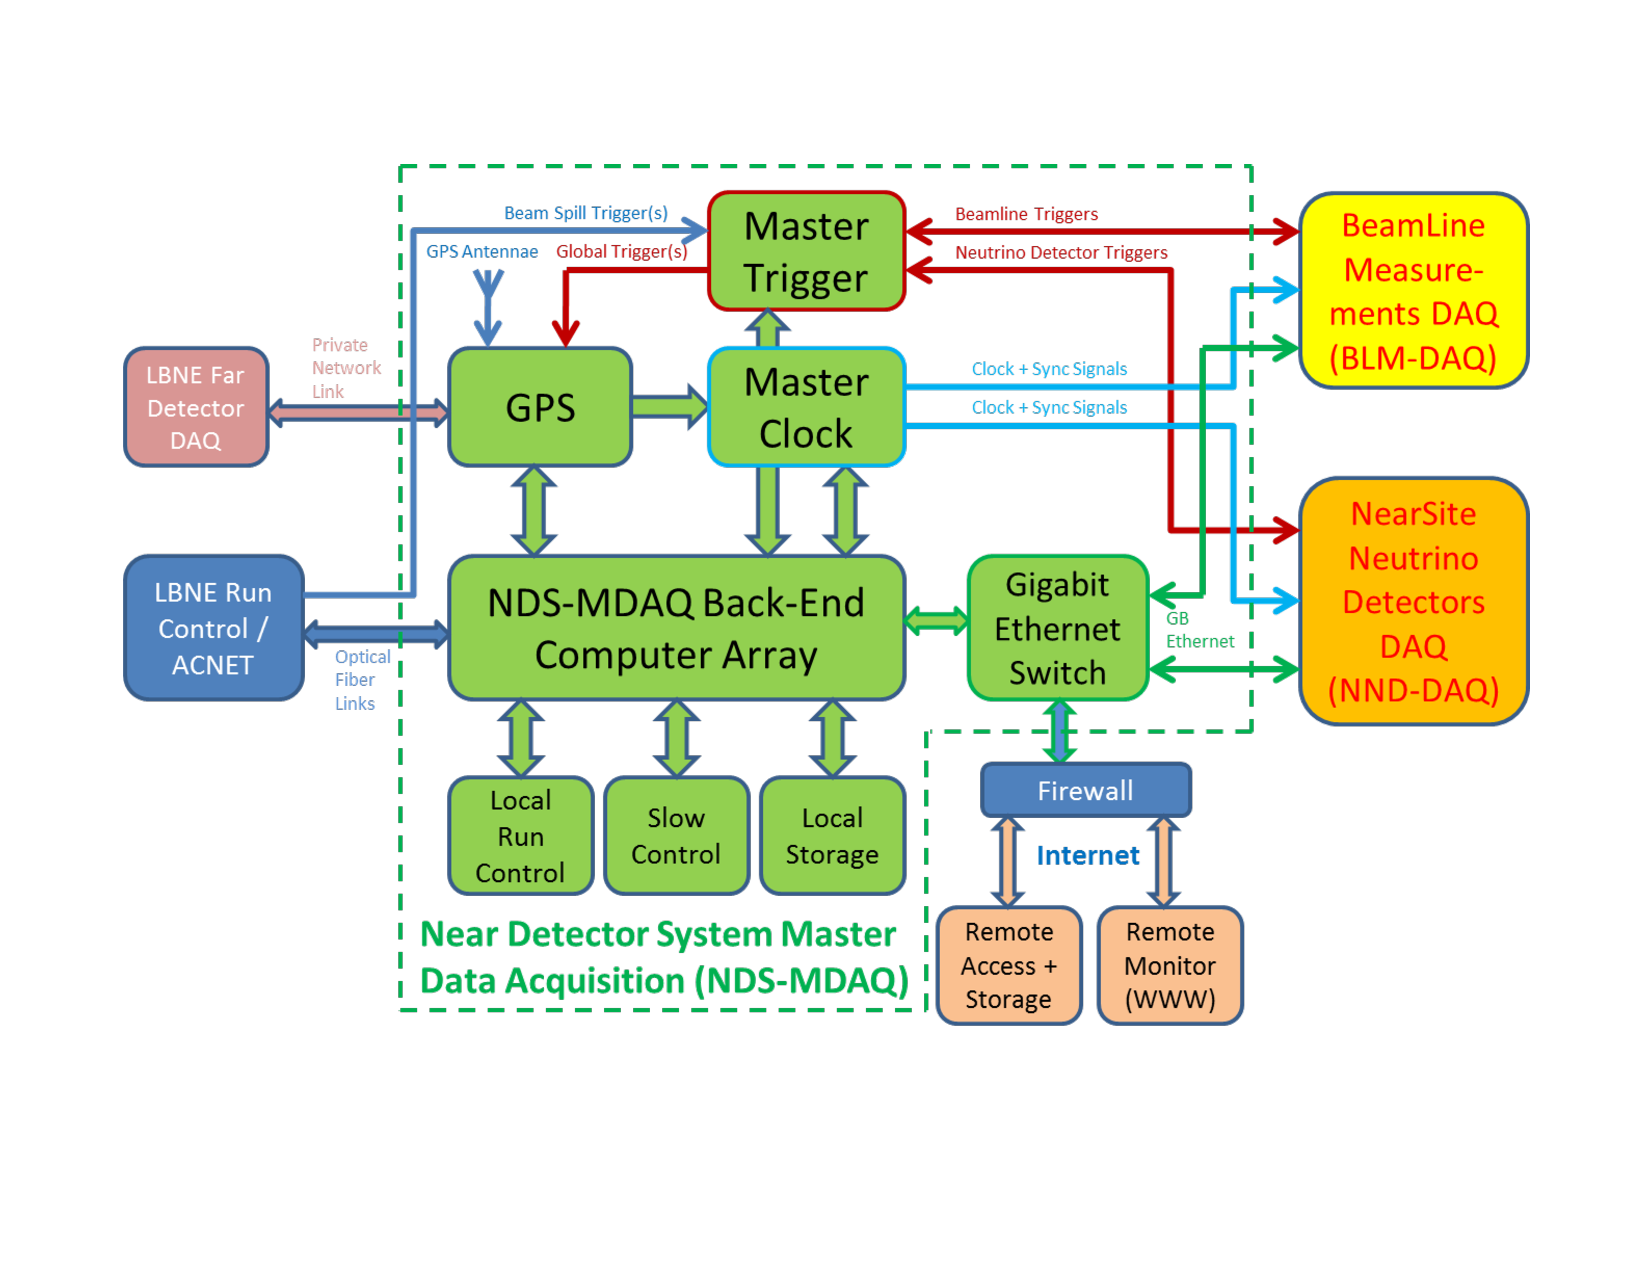
\includegraphics[width=6in,angle=0]{DAQ_Block}
\end{cdrfigure}

The NDS computing system encompasses two major activities: online computing (the required
slow-control systems \fixme{for what systems}) and offline computing for further development of the measurement 
strategy and for simulation work on technical systems. \fixme{why do we say `for further development of'? Why not just 
offline computing and simulation work?  Or is it only a portion of the offline computing?  Probably need to say how it 
interfaces with DUNE computing. It's just not clear as I read it.}

\subsection{NDS Master DAQ} % and Computing}
\label{sec:nd-master-daq}

The NDS-DAQ %design consists of equipment 
is designed to provide a high-level user interface 
for local run control and data taking, as well as for secure remote control and monitoring.   It will 
serve as the primary interface to the 
\begin{itemize}
\item slow-control system 
\item online data and DAQ performance monitoring  
\item raw data collection
\item building of events
\item data storage   
\end{itemize}
\fixme{It's not clear to me exactly what is `between all Near 
Neutrino Detector DAQs and Beamline Measurements DAQs.'}
%This (not sure what `this' is; am guessing it's the daq itself..)
The NDS-DAQ includes hardware triggering 
for two-way trigger processing between the NDS-DAQ \fixme{itself?} and all the NDS detectors, and 
\fixme{between itself and?} GPS for precision 
time-stamping and global clock synchronization.  It \fixme{The design?} is currently based on a channel count 
estimate of approximately 430,000 channels of neutrino detectors, plus $<1000$ channels of 
beamline detectors.  Custom electronics components for the NDS-DAQ are based on existing 
custom designs from other experiments, e.g,. T2K or ATLAS, \fixme{you can say ``they ARE based on X and Y'' or
``they WILL BE based on X or Y'' but not``they ARE based on X or Y'' } and %have all commercial 
implement commercial components for the trigger modules, clock and timing synchronization, GPS and environmental 
monitoring.

%The computing system encompasses two major activities: online computing with required 
%slow-control systems, and offline computing for further development of the measurement 
%strategy and for simulation work on technical systems. 
%The computing components are based 
%on currently available commercial computing and gigabit networking technology, which is 
%likely to improve over the next years without driving costs up for the final design.  

\fixme{I don't know why this section was for daq and computing. There's no explanation of how one leads
to the other or how they're related (I know they are!)}

\subsection{Beamline Measurements DAQ (BLM-DAQ)}

Similar to the NDS Master DAQ, the BLM-DAQ will mainly consist of a scalable back-end 
computer array, inter-connected to the individual beamline measurement detector DAQs via 
Gigabit Ethernet and specialized electronics modules for trigger processing and clock 
synchronization. 
\fixme{None of this is covered in the master daq section. I suspect that we need to retrieve some info
from the earlier version of this chapter when it was ``global daq''}
It interfaces to the NDS Master DAQ (NDS-MDAQ) for run control and global \fixme{want to use `global'?}
data collection. It will also have its own local run-control setup, consisting of a number 
of desktop workstations to allow independent local runs that include beamline measurement 
detectors only (useful during detector commissioning), calibration runs, stand-alone cosmic 
runs or other runs where the beam is stopped or not needed.


\section{NDS Computing}
\label{sec:nd-gdaq-global-computing}

The computing system encompasses two major activities: %The first is 
online computing (% which consists of 
the required slow-control systems) and %.  The second is 
offline 
computing which is costed off-Project, but is important to consider.
Offline computing is needed to complete 
the work outlined in the Measurement Strategy described in Chapter~\ref{ch:meas-strat} and the simulation work %important 
for the technical systems.
The computing components are based 
on currently available commercial computing and gigabit networking technology, which is 
likely to improve over the next years without driving costs up for the final design.  \fixme{There's no
mention of how the DAQ and the computing system are linked}


The required slow-control (online) computing systems will be defined when the Project moves 
from the conceptual-design to the preliminary-design phase.

For offline computing, resources are currently being provided by Fermilab, 
LANL and various universities.  Project-wide resources are currently 
being developed at Fermilab and Brookhaven.
